\documentclass[11pt]{beamer}
\setbeamercolor*{title}{fg=black}
\setbeamercolor*{frametitle}{fg=black}
\usepackage{graphicx}
\usepackage{polyglossia}
\setmainlanguage{russian}
\setmainfont{Times New Roman}
\setsansfont{Times New Roman}


\addtobeamertemplate{frametitle}{}{%
	\begin{picture}(0,0)
		\put(280,10){
\includegraphics[scale=0.05]{images/logo_osnovnoy_russkiy_chernyy.png}}
	\end{picture}
}
%Information to be included in the title page:
\title[About Beamer] %optional
{ Отзыв о посещении Государственного музея истории религии }


\author{Сиромашенко Владислав Романович}

\institute[VFU] % (optional)
{
	Факультет программнрой инженерии и компьютерной техники\\
	Университет ИТМО
}

\date[VLC 2026] % (optional)
{Март 2026}


\begin{document}
	\frame{\titlepage}
	
	\begin{frame}
		\frametitle{\textbf{Схема музея}}
		
		Уже на входе в музей, при рассмотрении схемы экспозиций я заметил интересную отсылку: православие и католичество расположены в параллельных залах, что похоже на параллельное развитие двух веток христианства в истории мира.
		
\includegraphics[width=0.8\textwidth]{low_images/shema.jpg}
	\end{frame}
	
	\begin{frame}
		\frametitle{\textbf{Временная выставка 1}}
		
		\begin{columns}[T] 
			\column{0.5\textwidth}
			Выставка посвящена Василию Ивановичу Грязнову, глубоко религиозному человеку, который в партнерстве с Я. И. Лабзиным смог построить в XIX веке Павлопасадску платочную мануфактуру. Предприятие было весьма успешное и добавило к образу русской женщины узорчатый платок.
			
			\column{0.5\textwidth}
			\centering
			
\includegraphics[width=0.8\textwidth, angle=-90]{low_images/Gryaznov.jpg}
			
\includegraphics[width=0.8\textwidth, angle=-90]{low_images/platok.jpg}
		\end{columns}
	\end{frame}
	
	\begin{frame}
		\frametitle{\textbf{Временная выставка 2}}
		
		\begin{columns}[T] 
			\column{0.5\textwidth}
			После же октябрьской революции начались гонения и на самих наследников основателей так и на церковь в этом регионе, т.к. Грязнов длительное время своей жизни участвовал в устроении Спасо-Преображенской Гуслицкой обители. За жизненные заслуги его хотели причислить к лику святых, но не успели сделать это до революции.
			
			
			\column{0.5\textwidth}
			\centering
			
\includegraphics[height=0.25\textheight, angle=-90]{low_images/409.jpg} 
			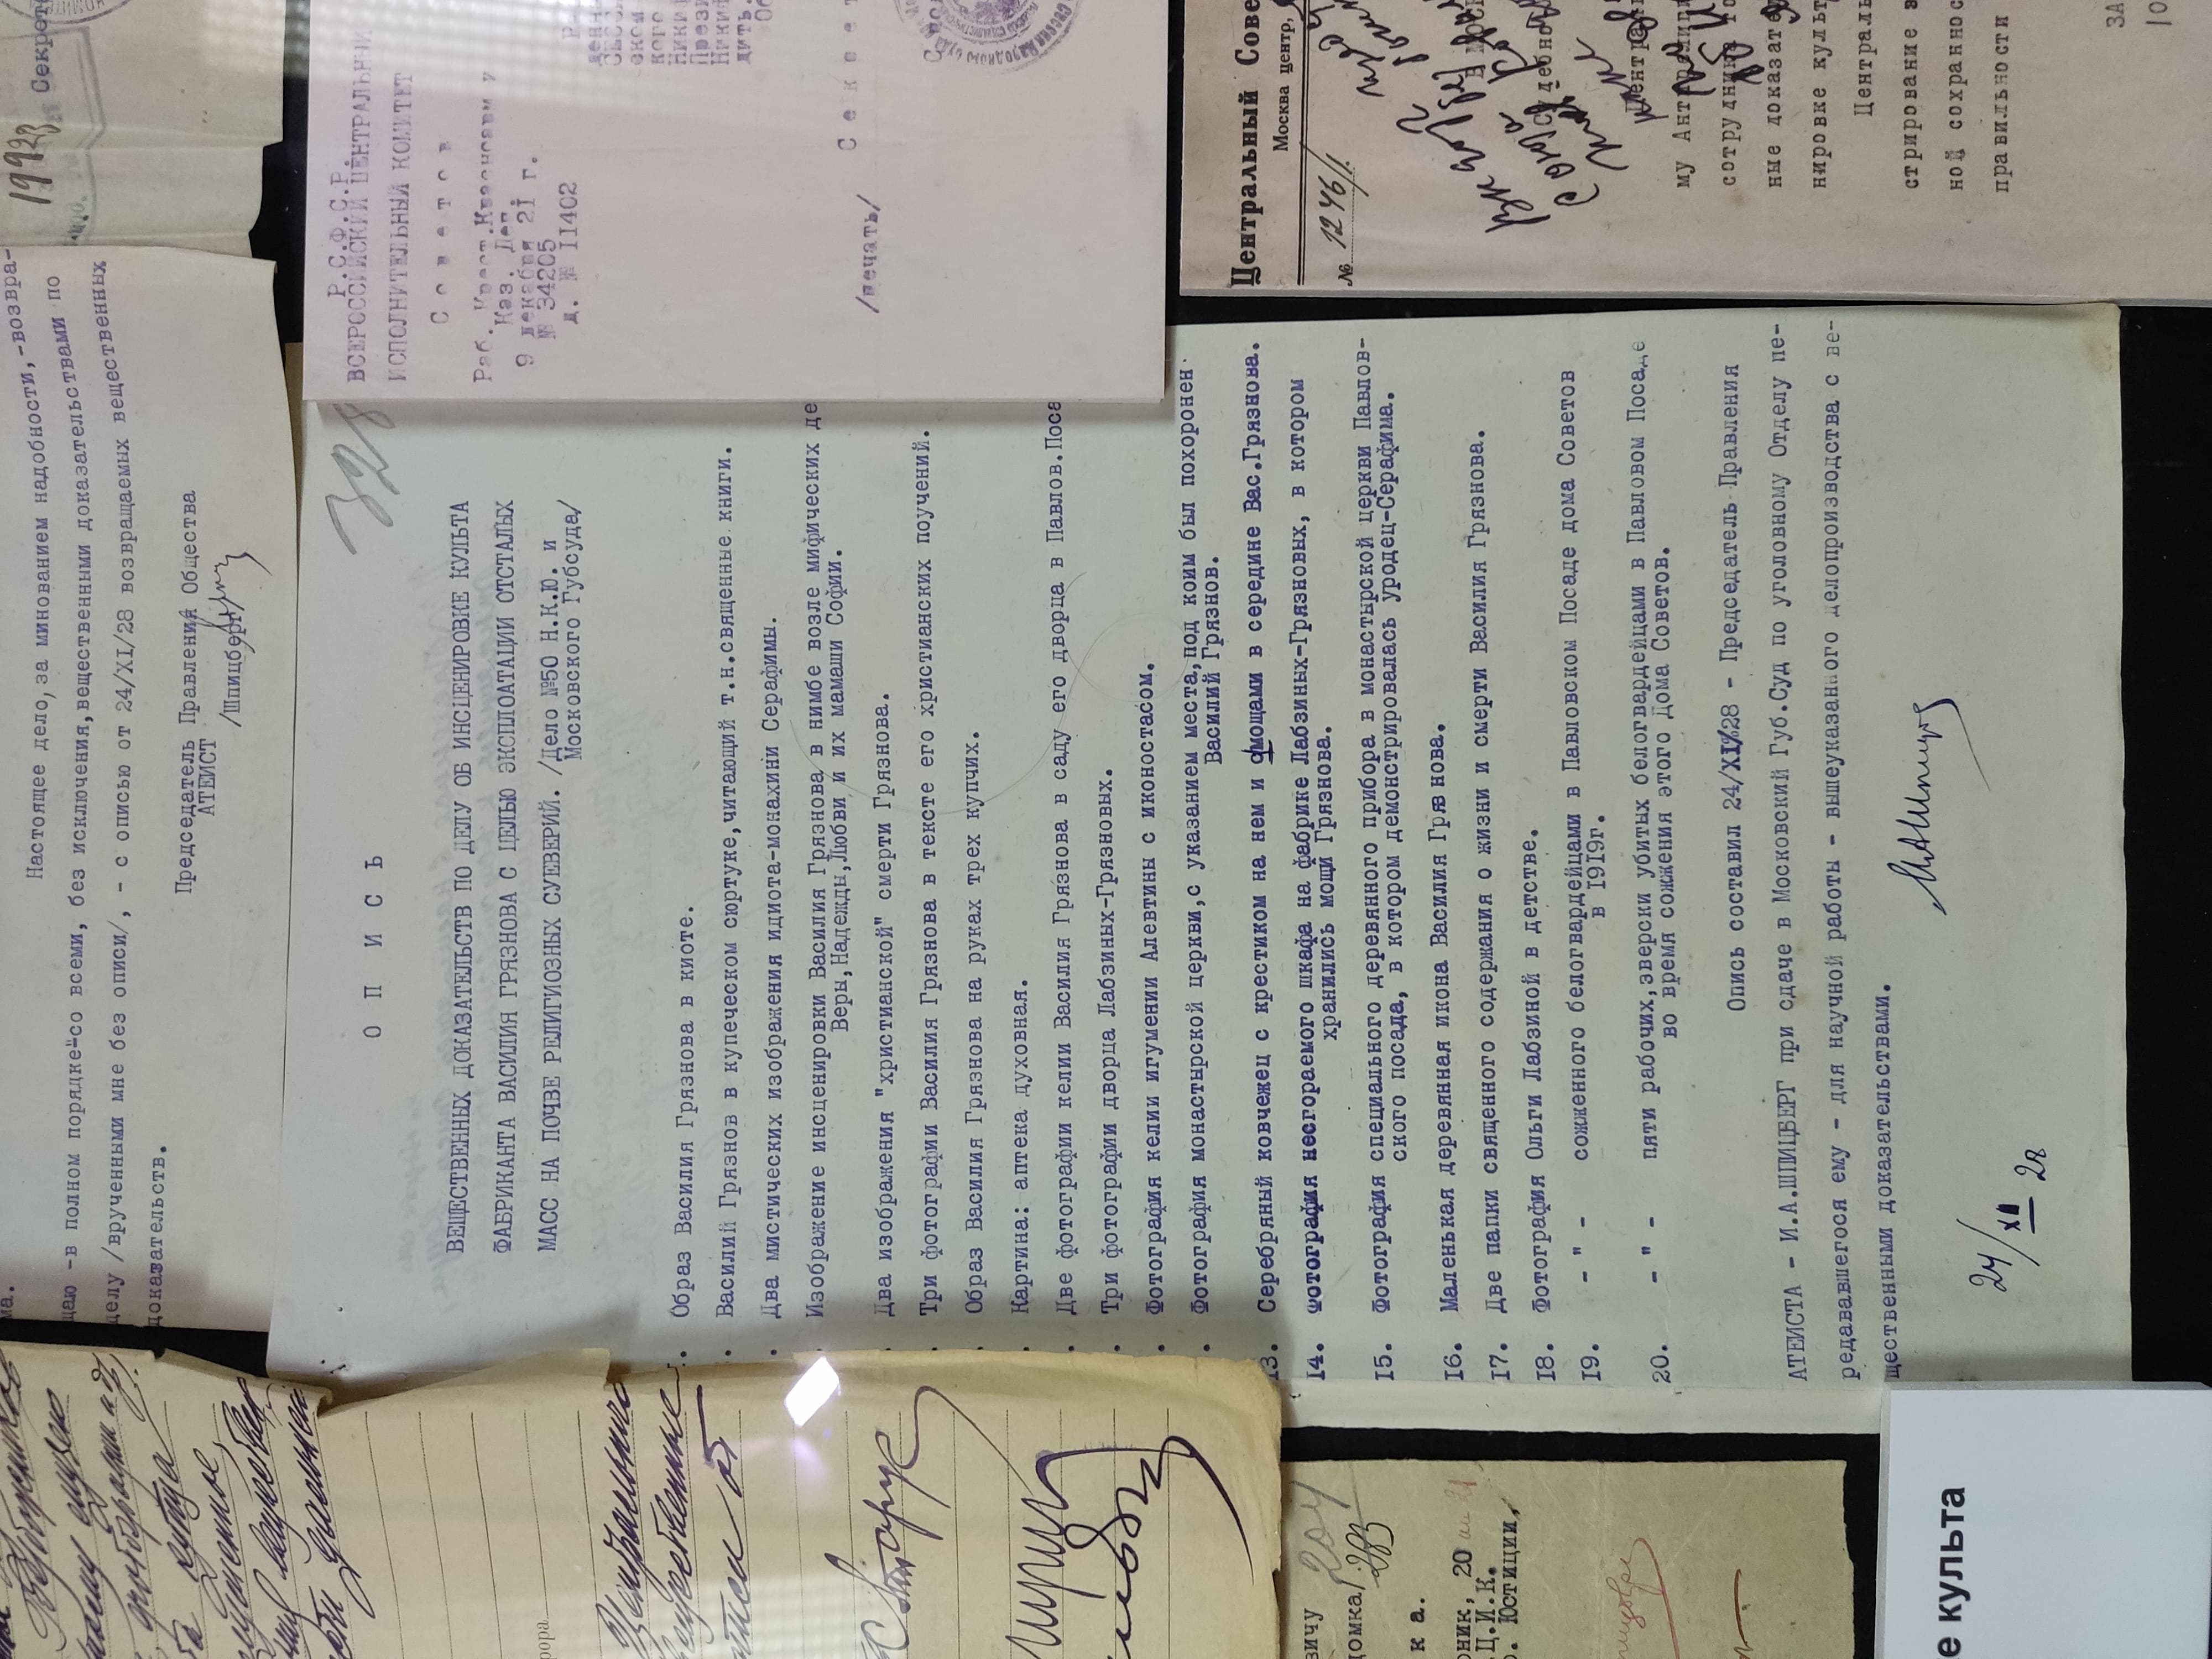
\includegraphics[height=0.25\textheight, angle=-90]{low_images/413.jpg} 
			Документы из судебных разбирательств
		\end{columns}
	\end{frame}
	
	\begin{frame}
		\frametitle{\textbf{Православие}}
			Одеяния и предметы представленные в этой части экспозиции дают понять, что церковь играла большую роль в жизни государства и могла позволить себе такое, но большинство предметов здесь из конца XIX века и я задумался о том, что , возможно, в начале 20-го века у церкви были некоторые трудности, если они не обновляли свой инвентарь. Возможно, просто в эту экспозицию не попали вещи "поновее".
			\centering {
\includegraphics[width=0.65\textwidth]{low_images/bogato.jpg}} 
	\end{frame}
	
	\begin{frame}
		\frametitle{\textbf{Борьба советов с церковью 1}}
		
		\begin{columns}[T] 
			\column{0.5\textwidth}
			Как я уже упоминал после Октябрьской революции началось активное гонение церкви. Гонение на церковь привязывали к гонению на капитал, аргументируя это тем, что буржуи вместе с церковью обворовывают рабочий класс
			
			\column{0.5\textwidth}
			\centering
			
\includegraphics[height=0.5\textheight, angle=-90]{low_images/chains.jpg}
		\end{columns}
	\end{frame}
	
	\begin{frame}
		\frametitle{\textbf{Борьба советов с церковью 2}}
		
		\begin{columns}[T] 
			\column{0.5\textwidth}
			\centering
			
\includegraphics[height=0.5\textheight]{low_images/tsar_pop_kulak.jpg}
			
			\column{0.5\textwidth}
			\centering
			
\includegraphics[height=0.5\textheight, angle=-90]{low_images/net.jpg}
		\end{columns}
	\end{frame}
	
	\begin{frame}
		\frametitle{\textbf{Борьба советов с церковью 3}}
		
		\begin{columns}[T] 
			\column{0.5\textwidth}
			\centering
			
\includegraphics[height=0.5\textheight, angle=-90]{low_images/boga_net.jpg}
			
			\column{0.5\textwidth}
			\centering
			
\includegraphics[height=0.5\textheight, angle=-90]{low_images/popilim.jpg}
		\end{columns}
	\end{frame}
	
	\begin{frame}
		\frametitle{\textbf{Борьба советов с церковью 4}}
		
		\begin{columns}[T] 
			\column{0.5\textwidth}
			\centering
			
\includegraphics[height=0.5\textheight]{low_images/fight.jpg}
			
			\column{0.5\textwidth}
			\centering
			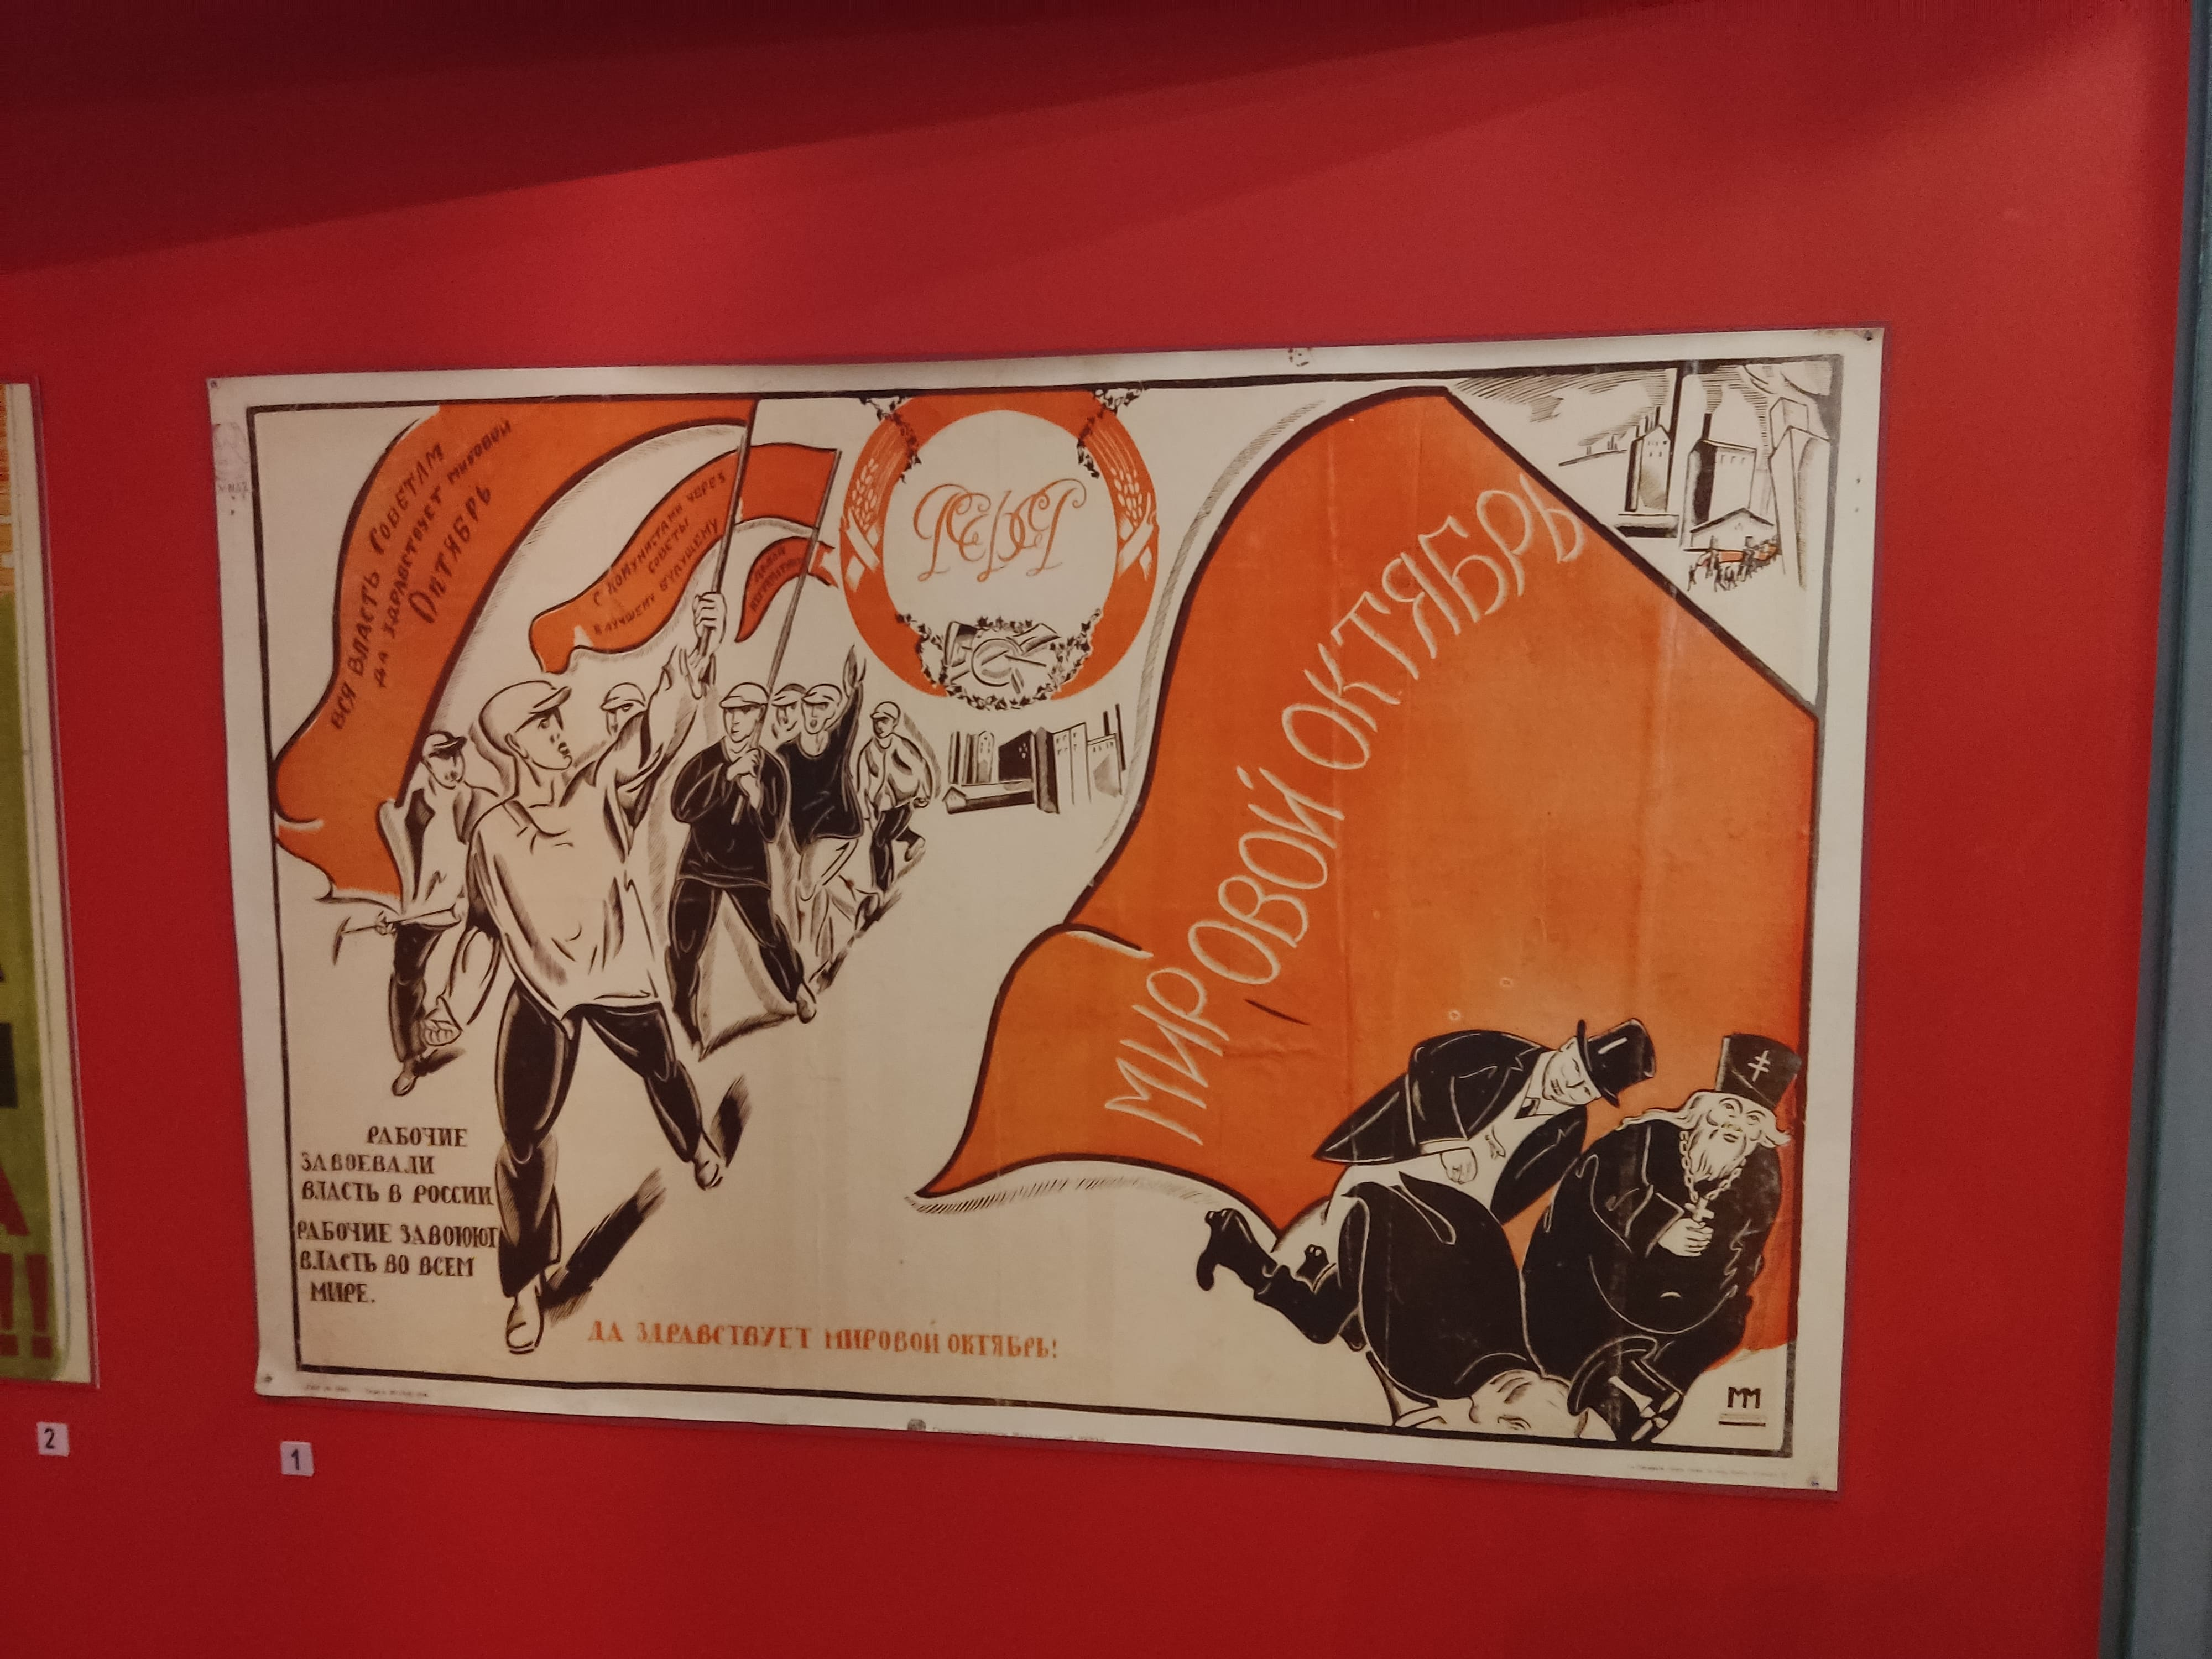
\includegraphics[height=0.5\textheight]{low_images/world_october.jpg}
		\end{columns}
		Всё это меня крайне расстроило. Ведь церковь никуда не ушла, а лишь ушла в подполье. Значит религия давала людям что-то чего не могли заменить советы, а лозунгами и гонениями ситуация не менялась. К тому же по Декрету СНК об отделении церкви от государства 1918 года устанавливалась свобода вероисповеданья, а действия власти противоречили этому постановлению.
	\end{frame}
	
	\begin{frame}
		\frametitle{\textbf{Католичество}}
		
		\begin{columns}[T] 
			\column{0.5\textwidth}
			Католическая церковь в XX веке тоже переживала кризис, связанный в основном со снижением роли церкви в жизни общества. На фото представлен Ватиканский собор, в котором принимались все основные решения. 
			
			\column{0.5\textwidth}
			\centering
			
\includegraphics[height=0.5\textheight, angle=-90]{low_images/vatican_sobor.jpg}
		\end{columns}
	\end{frame}
	
	
	\begin{frame}
		\frametitle{\textbf{Ислам}}
		
		\begin{columns}[T] 
			\column{0.5\textwidth}
			Несколько удивила исламская выставка. Чувствуется некая строгость в религиозных атрибутах. Предполагаю, что это также отражается на образе мыслей людей, исповедающих эту религию.
			
			\column{0.5\textwidth}
			\centering
			
\includegraphics[height=0.5\textheight, angle=-90]{low_images/alam.jpg}
		\end{columns}
	\end{frame}
	
	\begin{frame}
		\frametitle{\textbf{Ислам 2}}
		
		\begin{columns}[T] 
			\column{0.5\textwidth}
			\centering
			
\includegraphics[height=0.5\textheight, angle=-90]{low_images/plet.jpg}
			
			\column{0.5\textwidth}
			\centering
			
\includegraphics[height=0.5\textheight, angle=-90]{low_images/bulava.jpg}
		\end{columns}
	\end{frame}
	
	\begin{frame}
		\frametitle{\textbf{Выводы}}
		
		\begin{columns}[T] 
			\column{0.5\textwidth}
			Религия развивалась параллельно развитию цивилизаций и всегда так или иначе присутствовала в жизни людей. XX век не стал исключением, что наталкивает на мысль о том, что религия может давать свой уникальный "продукт", который пока не удается полностью заменить.  
			
			\column{0.5\textwidth}
			\centering
			
\includegraphics[height=0.5\textheight, angle=-90]{low_images/duma.jpg}
		\end{columns}
	\end{frame}
	
	\begin{frame}
		\frametitle{\textbf{Конец}}
		\centering
		Спасибо за внимание! 
		\newline \\
		
\includegraphics[height=0.65\textheight]{low_images/the_end.jpg}
	\end{frame}
\end{document}